\chapter{Experiment}\label{Experiment}

Nu we alle achterliggende theorie in hoofdstuk \ref{Lectuur} gezien hebben, kunnen we van start gaan met het experiment. Het doel van het experiment is aan de hand van enkele algemene technieken uit te Machine Learning een gevoelsanalyse uitvoeren op Nederlandse tekst, waarbij een algoritme het onderscheid aanleert tussen positief negatief. Het doel is om een algoritme te bekomen dat kan bepalen of een tekst een positieve of negatieve emotie uitdrukt. De prestatie van zo'n algoritme wordt in dit experiment beoordeeld op basis van de classificatieprecisie.  Wanneer het algoritme met een hoge precisie classificeert en bijna alle input correct kan classificeren als positief of negatief, dan spreken we van een goede prestatie. Wanneer de classificatieprecisie rond de 50\% of minder ligt, spreekt men van een slechte prestatie. Een classificatieprecisie van 50\% kan men vergelijken met een classificatiealgoritme dat telkens bij het bepalen van de output een munt gaat opgooien en op basis van kop of munt de output gaat bepalen. Wat neerkomt op het at random bepalen van de output.\\
%
Vooraleerst we de resultaten van het experiment bekijken, hebben we het in \ref{De Dataset} over de dataset die we gebruiken. Er is gekozen om gevoelsanalyse uit te voeren op film-, boek- en muziekrecensies. Waarom er is voor gekozen en hoe het verzamelen van de data is verlopen, wordt uitgelegd in deze sectie. In \ref{Naive Bayes Classifier met hetzelfde onderwerp voor trainings- en testset} en \ref{Naive Bayes Classifier met verschillend onderwerp voor trainings- en testset} volgen dan de experimenten en als laatste vatten we alle de bevindingen van het experiment samen in \ref{Conclusie experiment}.

\section{De Dataset}\label{De Dataset}

Zoals in de introductie staat vermeld waren film- ,boek- en muziekrecensies niet de eerste keuze. Eerst was het idee om de data van sociale media te nemen zoals tweets van Twitter. We zouden dan rond een bepaald onderwerp tweets verzamelen zoals bijvoorbeeld de nieuwe treinregeling van de NMBS. Omdat we voor het experiment gebruik maken van supervised learning technieken moesten we de tweets manueel labelen als positief of negatief om de tweets als trainingsset te kunnen gebruiken. Naast het feit dat het manueel labelen van de tweets een relatief intensief werk is, werd er ook opgemerkt dat er veel sarcasme heerst op Twitter. Voor bepaalde mensen is het al moeilijk om sarcasme te herkennen, voor een algoritme is dat zeker. Sarcastische tweets zijn onbruikbaar voor de training van de algoritmen en zorgen voor ruis in de dataset. De oplossing lag dan bij film-, muziek- en boekrecensies. Recensies bieden alles wat we nodig hebben. Een recensie is of wel positief, negatief of neutraal. Maar omdat er meestal een rating aanwezig is bij de review, is het gemakkelijk om automatisch te labelen en enkel de positieve en negatieve reviews op te nemen in onze dataset. De keuze om recensies te nemen over films, boeken en muziek was een beredeneerde keuze. Het aanbod is enorm, meestal niet te specifiek en toegankelijk. Merk op dat bij het verzamelen van de recensies gefocust werd op korte recensies van gebruikers en niet op de uitgebreide recensies van dagbladen. De recensies voor dit experiment zijn afkomstig van \url{moviemeter.nl}, \url{boekmeter.nl} en \url{muziekmeter.nl}. Deze websites waren de perfecte bron aan informatie. Ze bevatten allemaal toplijsten met films, boeken of muziekalbums waarop vele gebruikers hun persoonlijke mening plaatsen. Samen met die mening laten ze telkens ook een score op 5 achter, die het gevoel bij het betreffende item weerspiegelt. Perfect dus om de labeling van de meningen te automatiseren en een duidelijk onderscheid te maken tussen positieve en negatieve meningen. Voor datasets van de experimenten werden recensies met een score lager of gelijk aan twee op vijf beschouwd als negatief en recensies met een score gelijk of groter dan drie op vijf beschouwd als positief. De keuze van de grenzen is zo bepaald om een zo goed mogelijke spreiding te hebben van positieve en negatieve recensies. Moesten we bijvoorbeeld de score van vier of meer aannemen voor een positieve recensie dan zouden de recensies allemaal extreem positief zijn. Terwijl het ook interessant is om te kijken, hoe het algoritme omgaat met gematigde positieve recensies. Dit geeft ook het meeste algemene beeld van een gevoelsanalyse op Nederlandse tekst.  
\begin{figure}[h]%
    \centering
    \subfloat{{
\includegraphics[width=10cm]{voorbeeldrecensie} }}%
    \caption{Een voorbeeld van een positieve commentaar op \url{moviemeter.nl}}%
\end{figure}
\newline
Alle recensies zijn afkomstig van de ``All Time Top 250''-toplijst op de betreffende website. Door deze lijsten waren we zeker dat voldoende recensies aanwezig waren. Onderstaande tabel geeft het aantal verzamelde recensies van ieder onderwerp weer, waarbij een onderscheid wordt gemaakt tussen positief en negatief.\\

\begin{table}[h]
\centering
\begin{tabular}{l|l|l|l|}
\cline{2-4}
                                        & \textbf{Films} & \textbf{Muziek} & \textbf{Boeken} \\ \hline
\multicolumn{1}{|l|}{\textbf{Positief}} & 197358         & 15197           & 146             \\ \hline
\multicolumn{1}{|l|}{\textbf{Negatief}} & 17978          & 3019            & 3719            \\ \hline
\end{tabular}
\caption{Aantal verzamelende recensies} 
\end{table}

Wat meteen opvalt is dat er aanzienlijk minder positieve boekrecensies verzameld zijn. Hier zullen we rekening mee moeten houden tijdens het experiment. Voor de andere categorie\"en zijn de positieve recensies in grotere aantallen aanwezig dan de negatieve recensies, wat te maken heeft met dat we de ``All Time Top 250''-toplijst gebruiken voor zowel films, boeken als muziek als databron.
\newpage
\begin{figure}%
    \centering
    \subfloat{{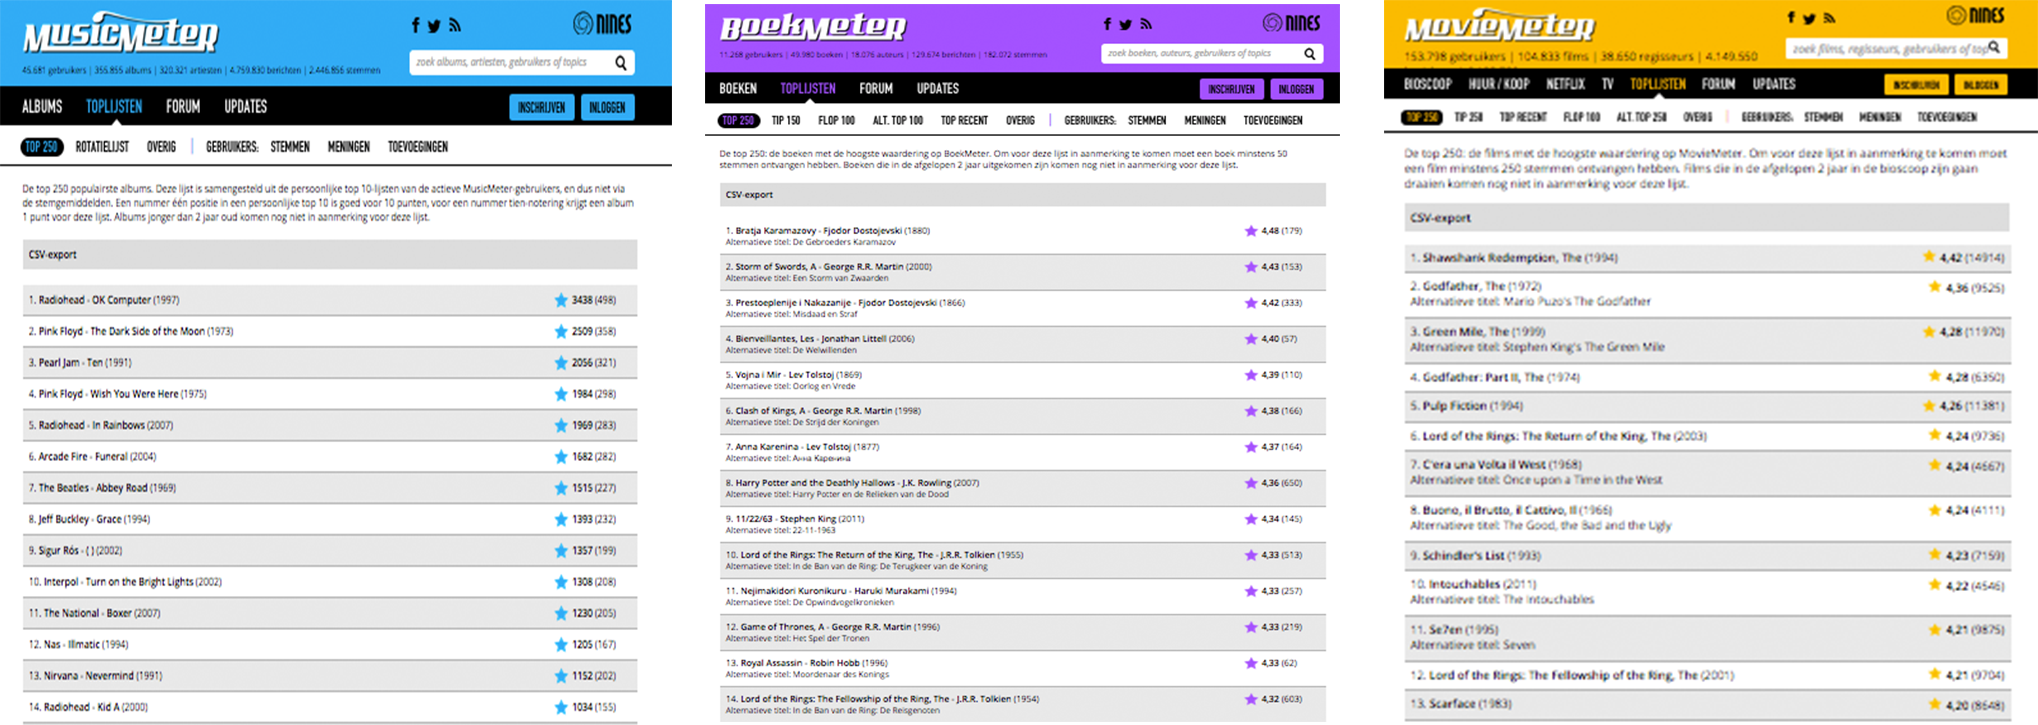
\includegraphics[width=15cm]{toplijsten} }}%
    \caption{de ``All Time Top 250''-toplijsten op de websites}%
\end{figure}

\section{Naive Bayes Classifier met hetzelfde onderwerp voor trainings- en testset}\label{Naive Bayes Classifier met hetzelfde onderwerp voor trainings- en testset}

Als eerste experiment gaan we kijken hoe de prestaties van een classifier zijn bij het trainen en testen met data van dezelfde soort. Bijvoorbeeld we trainen met een trainingsset van filmrecensies en testen het getrainde algoritme op een testset van filmrecensies. Dit gaan we voor zowel film-, boek- als muziekrecensies doen. Als classifier nemen we de Naive Bayes Classifier. Zoals vermeld in sectie \ref{Naive Bayes Classifier} is  dit een goede eerste keuze als leermethode. Verder geven we de data mee aan de classifier als een Bag of Words met TFIDF-weging.\\
%
Algemeen voor alle experimenten zijn de resultaten berekend als gemiddelde over dertig runs. Dit wil zeggen dat er telkens bij iedere run een nieuwe Naive Bayes Classifier wordt aangemaakt en vervolgens getraind en getest wordt met een andere trainings- en testset als de andere runs. Om te verzekeren dat bij elke run de trainingsset en testset verschillend zijn wordt bij iedere run de trainingsset en testset aangemaakt  door een bepaald aantal willekeurig uit de grote pool van recensies te selecteren. Na het uitvoeren van die runs wordt hier het gemiddelde van genomen. De resultaten van experimenten bestaan uit de classificatieprecisie van zowel de trainings- als testset, de standaard afwijking, de confusion matrix en het betrouwbaarheidsinterval voor 95\%. Het betrouwbaarheidsinterval wordt als \textit{(gemiddeld ; linkerlimiet ; rechterlimiet)} genoteerd. Een confusion matrix geeft aan hoeveel van elke outputmogelijkheid er juist zijn ge\"identificeerd door de classifier en hoeveel er fout als juist zijn ge\"identificeerd. Als laatste wordt er ook de learning curve bekeken om over- of underfitting uit te sluiten. De learning curve geeft het verloop van de precisie van de classifier weer voor de trainings- en validatieset. Op basis van het verloop en de ligging van de curve kan men detecteren of men te maken heeft met over- of underfitting. Figuur \ref{fig:highbias} en \ref{fig:highvariance} illustreren hoe men overfitting kan herkennen aan de hand van de learning curve. Merk op zowel de trainingsset als de testset altijd evenwichtig zijn verdeeld. Dit wil zeggen dat er telkens 1/2 van het totaal aantal samples bestaat uit positieve recensies en 1/2 uit negatieve recensies.
\newpage
\begin{figure}[h]
    \centering
    \subfloat{{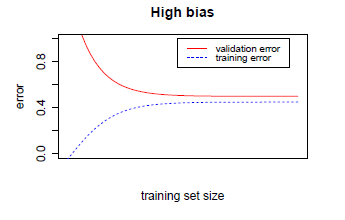
\includegraphics[width=5cm]{highbias}}}%
    \caption{Learning curve van een dataset met hoge bias. Wat duidt op underfitting [Bron: VUB-Cursus Machine Learning]}
    \label{fig:highbias}
 \end{figure}
 \begin{figure}[h]
 \centering
    \subfloat{{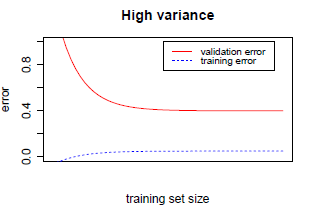
\includegraphics[width=5cm]{highvariance} }}%
    \caption{Learning curve van een dataset met hoge variantie. Wat duidt op overfitting [Bron: VUB-Cursus Machine Learning]}
    \label{fig:highvariance}
\end{figure}
\renewcommand\arraystretch{1.5}
\setlength\tabcolsep{0pt}
\begin{table}[h!]
\centering
\begin{tabular}{c >{\bfseries}r @{\hspace{0.7em}}c @{\hspace{0.4em}}c @{\hspace{0.7em}}l}
  \multirow{10}{*}{\parbox{1.1cm}{\bfseries\raggedleft eigelijke\\ waarde}} & 
    & \multicolumn{2}{c}{\bfseries voorspelde waarde} & \\
  & & \bfseries p & \bfseries n  \\
  & p$'$ & \MyBox{Waar}{Positief} & \MyBox{Vals}{Negatief}  \\[2.4em]
  & n$'$ & \MyBox{Vals}{Positief} & \MyBox{Waar}{Negatief} \\
\end{tabular}
\caption{Illustratie van de confusion matrix} 
\end{table}



\subsection{Filmrecensies als trainings- en testset}\label{Films als trainings- en testset}

Eerst trainen en testen we de Naive Bayes Classifier met filmrecensies. De trainingsset bestaat uit 6000 samples en de testset uit 2000 samples. Zoals eerder vermeld werden deze samples at random geselecteerd en is het volgende resultaat het gemiddelde van 30 runs.\\

\newpage\textbf{Standaard afwijking} = 0,0094\\
\textbf{95\% betrouwbaarheidsinterval} = (0,7064 ; 0,7030 ; 0,7101)\\

\begin{table}[h]
\centering
\setlength\tabcolsep{4pt}
\begin{minipage}[t]{0.48\textwidth}
\centering
\begin{tabular}{l|l|}
\cline{2-2}
                                            & \textbf{Precisie} \\ \hline
\multicolumn{1}{|l|}{\textbf{Trainingsset}} & 90,52\%           \\ \hline
\multicolumn{1}{|l|}{\textbf{Testset}}      & 70,66\%           \\ \hline
\end{tabular}
\caption{Classificatieprecisie Naive Bayes Classifier, getraind op filmrecensies}
\label{tab:movie-movie}
\end{minipage}%
\hfill
\begin{minipage}[t]{0.48\textwidth}
\centering
\begin{tabular}{lll}
                                 & \textbf{P}               & \textbf{N}               \\ \cline{2-3} 
\multicolumn{1}{l|}{\textbf{P'}} & \multicolumn{1}{l|}{824} & \multicolumn{1}{l|}{175} \\ \cline{2-3} 
\multicolumn{1}{l|}{\textbf{N'}} & \multicolumn{1}{l|}{410} & \multicolumn{1}{l|}{589} \\ \cline{2-3} 
\end{tabular}
\caption{Confusion matrix van de testset door de  Naive Bayes Classifier, getraind op filmrecensies} 
\label{tab:cm-movie-movie} 
\end{minipage}
\end{table}

Zoals men kan zien aan de resultaten zijn de prestaties goed. Een classificatieprecisie van 70\% voor een onbekende set met filmrecensies is een goede prestatie. Verder is het betrouwbaarheidsinterval heel klein, wat maakt dat we met 95\% kunnen zeggen dat de classificatie van filmrecensies door een Naive Baiyes Classifier, getraind op filmrecensies, met een precisie tussen 70\% en 71\% gebeurd. De confusion matrix geeft ons  ook een inzicht in wat er juist en fout geclassificeerd is. We zien dat de classifier overwegend beter positieve recensies kan identificeren dan negatieve.\\
%
Ten slotte wat we ook kunnen afleiden uit de cijfers, waar we zien dat zowel de test- als trainingsset goed presteren, zien we aan de learning curve dat we geen over- of underfitting hebben. 

\begin{figure}[h]%
    \centering
    \subfloat{{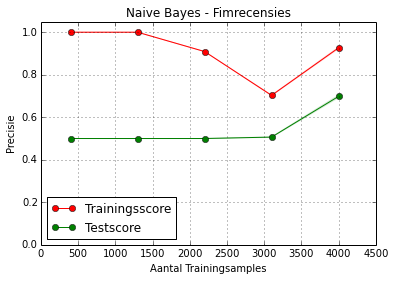
\includegraphics[width=5cm]{lc-movie-movie}}}%
    \label{fig:lc-movie-movie}
    \caption{Learning curve van de training van de Naive Bayes Classifier op filmrecensies}
\end{figure}

\subsection{Muziekrecensies als trainings- en testset}\label{Muziek als trainings- en testset}

Nu trainen en testen we de Naive Bayes Classifier met muziekrecensie. De trainingsset bestaat uit 6000 samples en de testset uit 2000 samples. Wederom werden deze samples at random geselecteerd en is het volgende resultaat het gemiddelde van 30 runs.\\

\textbf{Standaard afwijking} = 0,0096\\
\textbf{95\% betrouwbaarheidsinterval} = (0,8262 ; 0,8226 ; 0,8299)\\
 
\begin{table}[h]
\centering
\setlength\tabcolsep{4pt}
\begin{minipage}[t]{0.48\textwidth}
\centering
\begin{tabular}{l|l|}
\cline{2-2}
                                            & \textbf{Precisie} \\ \hline
\multicolumn{1}{|l|}{\textbf{Trainingsset}} & 93,44\%           \\ \hline
\multicolumn{1}{|l|}{\textbf{Testset}}      & 82,62\%           \\ \hline
\end{tabular}
\caption{Classificatieprecisie Naive Bayes Classifier, getraind op muziekrecensies}
\end{minipage}%
\hfill
\begin{minipage}[t]{0.48\textwidth}
\centering
\begin{tabular}{lll}
                                 & \textbf{P}               & \textbf{N}               \\ \cline{2-3} 
\multicolumn{1}{l|}{\textbf{P'}} & \multicolumn{1}{l|}{879} & \multicolumn{1}{l|}{120} \\ \cline{2-3} 
\multicolumn{1}{l|}{\textbf{N'}} & \multicolumn{1}{l|}{227} & \multicolumn{1}{l|}{772} \\ \cline{2-3} 
\end{tabular}
\caption{Confusion matrix van de testset door de  Naive Bayes Classifier, getraind op muziekrecensies} 
\end{minipage}
\end{table}

Hier zien we eveneens goede resultaten. Een classificatieprecisie van 82\% voor een onbekende set met muziekrecensies is eveneens een goede prestatie. Wederom is het betrouwbaarheidsinterval heel klein, wat maakt dat we met 95\% kunnen zeggen dat de classificatie van muziekrecensies door een Naive Baiyes Classifier, getraind op muziekrecensies, met een precisie van 82\% gebeurd. De confusion matrix toont ons opnieuw dat de classifier beter om kan met positieve recensies.
%
Wederom geeft onderstaande learning curve uitsluiting van over- of underfitting .

\begin{figure}[h]%
    \centering
    \subfloat{{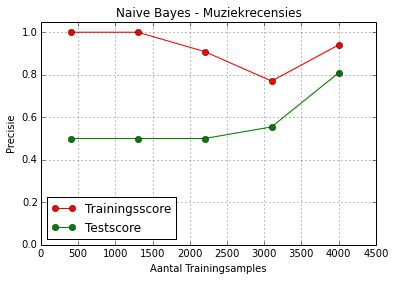
\includegraphics[width=5cm]{lc-music-music}}}%
    \label{fig:lc-music-music}
    \caption{Learning curve van de training van de Naive Bayes Classifier op muziekrecensies}
\end{figure}

\subsection{Boekrecensies als trainings- en testset}\label{Boeken als trainings- en testset}

Als laatste trainen en testen we de Naive Bayes Classifier met boekrecensies. De trainingsset bestaat uit 218 samples en de testset uit 74 samples. De samples zijn wederom at random geselecteerd en het resultaat is het gemiddelde van 30 runs.\\

\textbf{Standaard afwijking} = 0,0640\\
\textbf{95\% betrouwbaarheidsinterval} = (0,7176 ; 0,6932 ; 0,7419)\\
 
\begin{table}[h]
\centering
\setlength\tabcolsep{4pt}
\begin{minipage}[t]{0.48\textwidth}
\centering
\begin{tabular}{l|l|}
\cline{2-2}
                                            & \textbf{Precisie} \\ \hline
\multicolumn{1}{|l|}{\textbf{Trainingsset}} & 99,43\%           \\ \hline
\multicolumn{1}{|l|}{\textbf{Testset}}      & 71,76\%           \\ \hline
\end{tabular}
\caption{Classificatieprecisie Naive Bayes Classifier, getraind op boekrecensies}
\end{minipage}%
\hfill
\begin{minipage}[t]{0.48\textwidth}
\centering
\begin{tabular}{lll}
                                 & \textbf{P}               & \textbf{N}            \\ \cline{2-3} 
\multicolumn{1}{l|}{\textbf{P'}} & \multicolumn{1}{l|}{31} & \multicolumn{1}{l|}{5} \\ \cline{2-3} 
\multicolumn{1}{l|}{\textbf{N'}} & \multicolumn{1}{l|}{15} & \multicolumn{1}{l|}{21} \\ \cline{2-3} 
\end{tabular}
\caption{Confusion matrix van de testset door de  Naive Bayes Classifier, getraind op boekrecensies} 
\end{minipage}
\end{table}


Hier zien we ook goede resultaten. Een classificatieprecisie van 72\% voor een onbekende set met boekrecensies is een eveneens een goede prestatie. Hier zien we wel dat het betrouwbaarheidsinterval ruimer en is met 95\% zekerheid te zeggen, dat de classificatieprecisie zich tussen de 69\% en 74\% situeert, wat nog altijd acceptabel is. De confusion matrix toont ons opnieuw dat de classifier beter om kan met positieve recensies, al valt dit te nuanceren, aangezien we maar een hele klein pool hebben aan boekrecensies ten opzichte van de rest. Onderstaande learning curve sluit opnieuw over- en underfitting uit.\\
\newpage
\begin{figure}%
    \centering
    \subfloat{{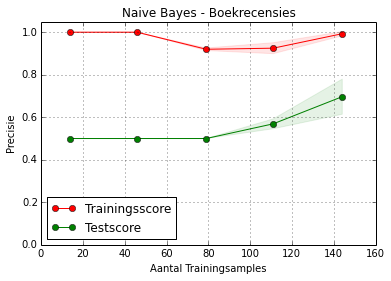
\includegraphics[width=5cm]{lc-boek-boek}}}%
    \label{fig:lc-boek-boek}
    \caption{Learning curve van de training van de Naive Bayes Classifier op boekrecensies}
\end{figure}

Nu we de prestaties weten van de Naive Bayes classifier met als trainings- en testset hetzelfde onderwerp. Kunnen we eens kijken wat de prestaties zijn met een verschillend onderwerp voor de trainingsset en testset.  

\section{Naive Bayes Classifier met een verschillend onderwerp voor trainings- en testset}\label{Naive Bayes Classifier met verschillend onderwerp voor trainings- en testset}

In \ref{Naive Bayes Classifier met hetzelfde onderwerp voor trainings- en testset} zagen we al dat de classificatie met een Naive Bayes Classifier, waarbij trainings- en testset tot hetzelfde onderwerp behoren, goede resultaten oplevert. Nu gaan we kijken of dit ook het geval is wanneer trainingsset en testset verschillend zijn. Wederom alle samples worden at random geselecteerd en de resultaten weerspiegelen telkens het gemiddelde van 30 runs.  

\subsection{Filmrecensies als trainingsset}\label{Filmrecensies als trainingsset}

Als eerste nemen we een getrainde Naive Bayes Classifier op filmrecensies en bekijken we de resultaten op een testset van muziek- en boekrecensies. De Naive Bayes Classifier is telkens getraind met 6000 samples.

\subsubsection{Muziekrecensies als testset}\label{Muziekrecensies als testset-movie}

De testset bestaat uit 2000 samples waarvan 1/2 positieve en 1/2 negatieve recensies.\\

\textbf{Standaard afwijking} = 0,01467\\
\textbf{95\% betrouwbaarheidsinterval} = (0,6207 ; 0,6152 ; 0,6263)\\
 
\begin{table}[h]
\centering
\setlength\tabcolsep{4pt}
\begin{minipage}[t]{0.48\textwidth}
\centering
\begin{tabular}{l|l|}
\cline{2-2}
                                            & \textbf{Precisie} \\ \hline
\multicolumn{1}{|l|}{\textbf{Testset}}      & 62,07\%           \\ \hline
\end{tabular}
\caption{Classificatieprecisie Naive Bayes Classifier, getraind op filmrecensies, getest op muziekrecensies}
\end{minipage}%
\hfill
\begin{minipage}[t]{0.48\textwidth}
\centering
\begin{tabular}{lll}
                                 & \textbf{P}               & \textbf{N}               \\ \cline{2-3} 
\multicolumn{1}{l|}{\textbf{P'}} & \multicolumn{1}{l|}{655} & \multicolumn{1}{l|}{345} \\ \cline{2-3} 
\multicolumn{1}{l|}{\textbf{N'}} & \multicolumn{1}{l|}{413} & \multicolumn{1}{l|}{586} \\ \cline{2-3} 
\end{tabular}
\caption{Confusion matrix van de testset ,bestaande uit muziekrecensies, door de  Naive Bayes Classifier, getraind op filmrecensies} 
\end{minipage}
\end{table}

De prestatie is minder dan de prestaties in \ref{Naive Bayes Classifier met hetzelfde onderwerp voor trainings- en testset}, maar 62\% is zeker aanvaardbaar. Ook het betrouwbaarheidsinterval is klein wat wil zeggen dat we  met 95\% zekerheid kunnen zeggen dat een Naive Bayes Classifier getraind op filmrecensies, muziekrecensies net 61\%-62\% precisie kan classificeren.  

\subsubsection{Boekrecensies als testset}\label{Boekrecensies testset-movie}

De testset bestaat uit 146 samples waarvan 1/2 positief en 1/2 negatief.\\

\textbf{Standaard afwijking} = 0,03714\\
\textbf{95\% betrouwbaarheidsinterval} = (0,6586 ; 0,6446 ; 0,6728)\\
 
\begin{table}[h]
\centering
\setlength\tabcolsep{4pt}
\begin{minipage}[t]{0.48\textwidth}
\centering
\begin{tabular}{l|l|}
\cline{2-2}
                                            & \textbf{Precisie} \\ \hline
\multicolumn{1}{|l|}{\textbf{Testset}}      & 65,87\%           \\ \hline
\end{tabular}
\caption{Classificatieprecisie Naive Bayes Classifier, getraind op filmrecensies, getest op boekrecensies}
\end{minipage}%
\hfill
\begin{minipage}[t]{0.48\textwidth}
\centering
\begin{tabular}{lll}
                                 & \textbf{P}               & \textbf{N}               \\ \cline{2-3} 
\multicolumn{1}{l|}{\textbf{P'}} & \multicolumn{1}{l|}{54} & \multicolumn{1}{l|}{18} \\ \cline{2-3} 
\multicolumn{1}{l|}{\textbf{N'}} & \multicolumn{1}{l|}{31} & \multicolumn{1}{l|}{41} \\ \cline{2-3} 
\end{tabular}
\caption{Confusion matrix van de testset, bestaande uit boekrecensies, door de  Naive Bayes Classifier, getraind op filmrecensies} 
\end{minipage}
\end{table}

De prestatie is in dezelfde lijn als de resultaten bij muziek. 

\subsection{Muziekrecensies als trainingsset}\label{Muziekrecensies als trainingsset}

Als tweede nemen we een getrainde Naive Bayes Classifier op muziekrecensies en bekijken we de resultaten op een testset van film- en boekrecensies. De Naive Bayes Classifier is telkens getraind met 6000 samples.

\subsubsection{Filmrecensies als testset}\label{Filmrecensies als testset}

De testset bestaat uit 2000 samples waarvan 1/2 positief en 1/2 negatief.\\

\textbf{Standaard afwijking} = 0,01146\\
\textbf{95\% betrouwbaarheidsinterval} = (0,6107 ; 0,6063 ; 0,6150)
 
\begin{table}[h]
\centering
\setlength\tabcolsep{4pt}
\begin{minipage}[t]{0.48\textwidth}
\centering
\begin{tabular}{l|l|}
\cline{2-2}
                                            & \textbf{Precisie} \\ \hline
\multicolumn{1}{|l|}{\textbf{Testset}}      & 61,07\%           \\ \hline
\end{tabular}
\caption{Classificatieprecisie Naive Bayes Classifier, getraind op muziekrecensies, getest op filmrecensies}
\end{minipage}%
\hfill
\begin{minipage}[t]{0.48\textwidth}
\centering
\begin{tabular}{lll}
                                 & \textbf{P}               & \textbf{N}               \\ \cline{2-3} 
\multicolumn{1}{l|}{\textbf{P'}} & \multicolumn{1}{l|}{691} & \multicolumn{1}{l|}{308} \\ \cline{2-3} 
\multicolumn{1}{l|}{\textbf{N'}} & \multicolumn{1}{l|}{469} & \multicolumn{1}{l|}{530} \\ \cline{2-3} 
\end{tabular}
\caption{Confusion matrix van de testset ,bestaande uit filmrecensies, door de  Naive Bayes Classifier, getraind op muziekrecensies} 
\end{minipage}
\end{table}

De resultaten zijn aanvaardbaar met een classificatieprecisie van 61\% en een klein betrouwbaarheidsinterval van 95\%.

\subsubsection{Boekrecensies als testset}\label{Boekrecensies als testset}

De testset bestaat uit 146 samples waarvan 1/2 positief en 1/2 negatief.\\

\textbf{Standaard afwijking} = 0,03519\\
\textbf{95\% betrouwbaarheidsinterval} = (0,6146 ; 0,6012 ; 0,6280)
 
\begin{table}[h]
\centering
\setlength\tabcolsep{4pt}
\begin{minipage}[t]{0.48\textwidth}
\centering
\begin{tabular}{l|l|}
\cline{2-2}
                                            & \textbf{Precisie} \\ \hline
\multicolumn{1}{|l|}{\textbf{Testset}}      & 61,46\%           \\ \hline
\end{tabular}
\caption{Classificatieprecisie Naive Bayes Classifier, getraind op muziekrecensies, getest op boekrecensies}
\end{minipage}%
\hfill
\begin{minipage}[t]{0.48\textwidth}
\centering
\begin{tabular}{lll}
                                 & \textbf{P}               & \textbf{N}               \\ \cline{2-3} 
\multicolumn{1}{l|}{\textbf{P'}} & \multicolumn{1}{l|}{43} & \multicolumn{1}{l|}{29} \\ \cline{2-3} 
\multicolumn{1}{l|}{\textbf{N'}} & \multicolumn{1}{l|}{26} & \multicolumn{1}{l|}{46} \\ \cline{2-3} 
\end{tabular}
\caption{Confusion matrix van de testset, bestaande uit boekrecensies, door de  Naive Bayes Classifier, getraind op muziekrecensies} 
\end{minipage}
\end{table}


Een gelijkaardige prestatie als filmrecensies, met een gemiddelde classificatieprecisie van 61\% en eveneens een klein betrouwbaarheidsinterval van 95\%.

\subsection{Boekrecensies als trainingsset}\label{Boekrecensies als trainingsset}

Als laatste nemen we een getrainde Naive Bayes Classifier op boekrecensies en bekijken we de resultaten op een testset van film- en muziekrecensies. De Naive Bayes Classifier is telkens getraind met 276 samples.


\subsubsection{Filmrecensies als testset}\label{Filmrecensies als testset}

De testset bestaat uit 2000 samples waarvan 1/2 positief en 1/2 negatief.\\

\textbf{Standaard afwijking} = 0,01812\\
\textbf{95\% betrouwbaarheidsinterval} = (0,5625 ; 0,5556 ; 0,5693)
 
\begin{table}[h]
\centering
\setlength\tabcolsep{4pt}
\begin{minipage}[t]{0.48\textwidth}
\centering
\begin{tabular}{l|l|}
\cline{2-2}
                                            & \textbf{Precisie} \\ \hline
\multicolumn{1}{|l|}{\textbf{Testset}}      & 56,25\%           \\ \hline
\end{tabular}
\caption{Classificatieprecisie Naive Bayes Classifier, getraind op boekrecensies, getest op filmrecensies}
\end{minipage}%
\hfill
\begin{minipage}[t]{0.48\textwidth}
\centering
\begin{tabular}{lll}
                                 & \textbf{P}               & \textbf{N}               \\ \cline{2-3} 
\multicolumn{1}{l|}{\textbf{P'}} & \multicolumn{1}{l|}{539} & \multicolumn{1}{l|}{460} \\ \cline{2-3} 
\multicolumn{1}{l|}{\textbf{N'}} & \multicolumn{1}{l|}{414} & \multicolumn{1}{l|}{585} \\ \cline{2-3} 
\end{tabular}
\caption{Confusion matrix van de testset ,bestaande uit filmrecensies, door de  Naive Bayes Classifier, getraind op boekrecensies} 
\end{minipage}
\end{table}

Met 56\% kunnen we spreken van een slechte prestatie. Net iets meer dan de helft van de classificaties wordt juist geclassificeerd. Het betrouwbaarheidsinterval is ook klein, wat betekent dat we met 95\% zekerheid kunnen zeggen dat de classificatieprecisie zich tussen 56\% - 57\% situeert. Wat nogmaals de slechte prestatie bevestigd.

\subsubsection{Muziekrecensies als testset}\label{Muziekrecensies als testset}

De testset bestaat uit 2000 samples waarvan 1/2 positief en 1/2 negatief.\\
\textbf{Standaard afwijking} = 0,01448\\
\textbf{95\% betrouwbaarheidsinterval} = (0,5647 ; 0,5592, 0,5702)

\begin{table}[h]
\centering
\setlength\tabcolsep{4pt}
\begin{minipage}[t!]{0.48\textwidth}
\centering
\begin{tabular}{l|l|}
\cline{2-2}
                                            & \textbf{Precisie} \\ \hline
\multicolumn{1}{|l|}{\textbf{Testset}}      & 56,47\%           \\ \hline
\end{tabular}
\caption{Classificatieprecisie Naive Bayes Classifier, getraind op boekrecensies, getest op muziekrecensies}
\end{minipage}%
\hfill
\begin{minipage}[t!]{0.48\textwidth}
\centering
\begin{tabular}{lll}
                                 & \textbf{P}               & \textbf{N}               \\ \cline{2-3} 
\multicolumn{1}{l|}{\textbf{P'}} & \multicolumn{1}{l|}{604} & \multicolumn{1}{l|}{395} \\ \cline{2-3} 
\multicolumn{1}{l|}{\textbf{N'}} & \multicolumn{1}{l|}{475} & \multicolumn{1}{l|}{524} \\ \cline{2-3} 
\end{tabular}
\caption{Confusion matrix van de testset, bestaande uit muziekrecensies, door de  Naive Bayes Classifier, getraind op boekrecensies} 
\end{minipage}
\end{table}

Een classificatieprecisie van 56\% is niet goed. Dit is analoog als bij voorgaande sectie met als testset filmrecensies\\

De resultaten op muziek- en filmrecensies zijn met 56\%, minder als de vorige in \ref{Filmrecensies als trainingsset} en \ref{Muziekrecensies als testset}, waar we rond de 60\% liggen.

\section{Conclusie experiment}\label{Conclusie experiment}

Nu we alle mogelijke combinaties van training en testing hebben uitgevoerd is het interessant om alle resultaten naast elkaar te leggen. Onderstaande tabel geeft nog eens alle classificatiescores in een kruistabel weer.

\begin{table}[h]
\centering
\begin{tabular}{l|c|c|c|}
\cline{2-4}
                                      & \textbf{Films} & \textbf{Muziek} & \textbf{Boeken} \\ \hline
\multicolumn{1}{|l|}{\textbf{Films}} & 70,66\%         & 61,00\%         & 56,25\%         \\ \hline
\multicolumn{1}{|l|}{\textbf{Muziek}} & 62,07\%         & 82,62\%         & 56,47\%         \\ \hline
\multicolumn{1}{|l|}{\textbf{Boeken}} & 65,87\%         & 61,46\%         & 71,76\%         \\ \hline
\end{tabular}
\label{tab:alles}
\caption{Kruistabel van alle classificatieresultaten uit \ref{Naive Bayes Classifier met verschillend onderwerp voor trainings- en testset} en \ref{Naive Bayes Classifier met hetzelfde onderwerp voor trainings- en testset} met de kolommen het onderwerp van de trainingsset en de rijen het onderwerp van de testset.} 
\end{table}


Op basis van de tabel kunnen we zeggen dat het trainen en testen met het zelfde onderwerp het beste resultaat geeft. Verder presteren muziek en films goed op een vreemde testset. Hierbij bedoelen we een testset die over een andere onderwerp gaat dan waar het algoritme op getraind is.  Boeken presteren hier minder. Dit kan te wijten zijn aan de kleinere dataset, waardoor er een bias of voorkeur ontstaat op bijvoorbeeld auteursnamen. Die bias op auteursnamen kan helpen bij het classificeren van boeken om positieve of negatieve recensies te herkennen, maar gaat niet helpen in de classificatie van een set over een ander onderwerp. Ook de prestatie van muziek springt in het oog met meer dan 10\% verschil tussen de andere classifiers met de trainingsset en testset over hetzelfde onderwerp. Maar het daalt wel 20\% wanneer het een vreemde set moet classificeren. Dit duidt eveneens op een bias of voorkeur op een bepaald feature die specifiek is voor muziek waardoor het classificeren van muziekrecensies veel beter gaat. Nog een interessant inzicht is dat filmrecensies een goede trainingsset blijken te zijn voor boekrecensies.  Ondanks de kleine dataset van boeken, kunnen we toch aan de hand van het betrouwbaarheidsinterval met 95\% zekerheid zeggen dat een getrainde Naive Bayes Classifier op filmrecensies, boekrecensies met een precisie tussen de 64\% en 67\% zal classificeren.\\

Nog een andere manier om de resultaten bij elkaar te leggen, is het bekijken van de confusion matrixen. We kunnen hier een percentueel gemiddelde van nemen en kijken hoe gemiddeld de classificatie verloopt bij sectie \ref{Naive Bayes Classifier met hetzelfde onderwerp voor trainings- en testset} waar de sets over hetzelfde onderwerp zijn en sectie \ref{Naive Bayes Classifier met verschillend onderwerp voor trainings- en testset}, waar ze verschillend zijn.

\begin{table}[h]
\centering
\setlength\tabcolsep{4pt}
\begin{minipage}[t]{0.48\textwidth}
\centering
\begin{tabular}{lll}
                                 & \textbf{P}               & \textbf{N}               \\ \cline{2-3} 
\multicolumn{1}{l|}{\textbf{P'}} & \multicolumn{1}{l|}{43\%} & \multicolumn{1}{l|}{6\%} \\ \cline{2-3} 
\multicolumn{1}{l|}{\textbf{N'}} & \multicolumn{1}{l|}{18\%} & \multicolumn{1}{l|}{31\%} \\ \cline{2-3} 
\end{tabular}
\caption{Gemiddelde confusion matrix in percent voor een Naive Bayes Classifier, waar trainings- en testset over hetzelfde onderwerp gaan}
\end{minipage}%
\hfill
\begin{minipage}[t]{0.48\textwidth}
\centering
\begin{tabular}{lll}
                                 & \textbf{P}               & \textbf{N}               \\ \cline{2-3} 
\multicolumn{1}{l|}{\textbf{P'}} & \multicolumn{1}{l|}{32\%} & \multicolumn{1}{l|}{18\%} \\ \cline{2-3} 
\multicolumn{1}{l|}{\textbf{N'}} & \multicolumn{1}{l|}{21\%} & \multicolumn{1}{l|}{29\%} \\ \cline{2-3} 
\end{tabular}
\caption{Gemiddelde confusion matrix in percent voor een Naive Bayes Classifier, waar trainings- en testset over een verschillend onderwerp gaan} 
\end{minipage}
\end{table}


Voor beide matrixen, ziet men duidelijk dat positieve recensies beter ge\"identificeerd worden. Na het herbekijken van de datasets, is een mogelijk verklaring dat mensen zich bij een positieve recensie zich veel expressiever en uitgebreider uitdrukken dan bij een negatieve recensie. Hierdoor krijgt de classifier meer informatie over de features van een positief document waardoor het beter het concept ``Positief'' kan bepalen 
